\documentclass[11pt,a4paper,notitlepage,onecolumn,twoside]{article}

\usepackage{amsmath}
\usepackage{amssymb}
\usepackage{amsthm}
\usepackage{graphicx}
\usepackage{verbatim}

\newtheorem{definition}{Definition}
\newtheorem{example}{Example}
\newtheorem{formula}{Formula}
\newtheorem{problem}{Problem}

\setlength\parindent{0pt}

\title{Identity on the Web \\ Notes}
\author{Wouter Beek \and Stefan Schlobach \and Frank van Harmelen}

\begin{document}

\maketitle

\section{Abstract}

Identity relations are at the foundation of the Linked Open Data initiative and on the Semantic Web in general. They allow the interlinking of alternative descriptions of the same thing. However, the traditional notion of identity (owl:sameAs) is often problematic, e.g. when objects are considered the same in some contexts but not in others. The standing practice in such cases is to use weaker relations of relatedness (e.g. skos:related). Unfortunately, this limits reasoners in drawing inferences. 

We propose a method that treats a given identity relation as a collection of indiscernability pairs, assigning meaning to such relations in terms of shared properties/values. Reflexivity, symmetry and (in some cases) transitivity are preserved under indiscernability, allowing reasoners to infer new results.

Reinterpreting identity in this way allows the calculation of upper and a lower bounds, turning crisp identity into rough indiscernability, based on the well-understood rough-set semantics. These rough sets can be used to provide automated assistance for finding false positive and false negative errors for existing linksets.

In a series of experiments we show that this method can indeed be used to improve on linksets that are the result of state of the art automated alignment mappings.

\section{Introduction}

Identity is a problem on the Web. It is a very strong notion when used in an open world context. Using non-identity relations to assert notions of similarity hampers reasoning and often does not explain the aspects with respect to which similarity is asserted.\footnote{There is an indeterminate number of ways which two objects can be considered similar.}

\section{Identity}

According to the standard definition, $a$ and $b$ are identical iff they co-designate [REF]. Co-designation is often cyclicly defined in terms of indiscernability. The principle of the indiscernability of identicals (also known as Leibniz's Law) is given in \ref{eq:leibniz_law}.

\begin{formula}[Leibniz' Law]
\label{eq:leibniz_law}
$\forall a,b: a = b \rightarrow \forall \phi: \phi(a) \leftrightarrow \phi(b)$
\end{formula}

The converse of the principle of the indiscernability of identicals is \emph{the principle of the identity of indiscernables}, given in \ref{eq:principle_of_the_identity_of_indiscernables}. This principle is vacuously true, since for every $x$ in the domain, \emph{identical-to-$x$} is a unary predicate.

\begin{formula}[Principle of the identity of indiscernables]
\label{eq:principle_of_the_identity_of_indiscernables}
$\forall a,b: \forall \phi: \phi(a) \leftrightarrow \phi(b) \rightarrow a = b$
\end{formula}

The substitutivity of identicals \ref{eq:substitutivity_principle} does not hold for intensional meanings (e.g., \ref{eq:hespherus_phosphorus}) or for modal contexts (e.g., \ref{eq:substitution_modality}).

\begin{formula}[Substitutivity principle]
\label{eq:substitutivity_principle}
$a = b \rightarrow \phi \rightarrow [a \\ b]\phi$
\end{formula}

\begin{example}[Substitution of intensions]
\begin{subequations}
\label{eq:hespherus_phosphorus}
\begin{align}
\text{Hesperus contains eight letters.}\\
\text{Phosphorus contains eight letters.\footnote{Hespherus is the Evening Star; Phosphorus is the Morning Star.}}
\end{align}
\end{subequations}
\end{example}

\begin{example}[Substitution under modality]
\begin{subequations}
\label{eq:substitution_modality}
\begin{align}
\text{It is a necessary truth that 9 is larger than 7.}\\
\text{It is a necessary truth that 9 is the number of planets.\footnote{Pluto, anyone?}}
\end{align}
\end{subequations}
\end{example}

The relevance of the substitutivity principle to the identity relation is unclear to me, since it only seems to restrict the number of deductions that involve identity. It does not seem to touch on the validity of the identity relation itself.

\section{Indiscernability}

Another definition of the identity relation is that it is the smallers equivalence relation.

Indiscernability is a weaker notation than identity. It is defined using a subset of the properties.

\begin{definition}[Indiscernability relative to a set of properties $\Phi$]
\begin{equation}
x \approx b \  \text{iff} \  \forall \phi \in \Phi (\phi(x) \leftrightarrow \phi(y))
\end{equation}
\end{definition}

Any relation that satisfies the following restriction is a similarity relation:

\begin{definition}[Similarity]
\begin{align}
R(x) \subseteq S(x) \\
y \in S(x) \rightarrow R(y) \subseteq S((x)
\end{align}
\end{definition}

In other words, similarity is a grouping if indiscernability.

\section{Identity on the Web}

Existing literature:
(1) A replacement of identity with similarity.
(2) A 

\begin{problem}
Some properties express propositions $\phi$ while others express aspects of formulations of propositions (e.g., ``this encoding of $\phi$ was asserted by agent $A$'') or labels/literal that are not identical but that do not necessarily conflict (e.g., two descriptions of a resource that are formulated in different natural languages but that do have the same meaning).

The indiscernability that comes with an identity relation is restricted to properties that express propositions.
\end{problem}

\begin{problem}
In practice we come accross notational differences for typed literals that are intended to have the same meaning, but that are asserted using different datatype URIs. E.g., \texttt{8^^xsd:decimal} and \texttt{8.0^^xsd:float}; or even \texttt{8cm''^^xsd:string}.
\end{problem}

\begin{problem}
The same property may be expressed in different ways due to the use of existential quantification. For instance,
$\exists x: Length(o, x) \land Value(x, \texttt{80^^xsd:int}) \land Scale(x, \texttt{``mm''^^xsd:string})$ has the same meaning as $Length(o, \texttt{``80mm''^^xsd:string})$.
\end{problem}

\section{Approach I}

We define the shared properties of two individuals.

\begin{definition}[Shared predicates]
\label{def:shared_predicates}
\begin{equation}
\mathbb{P}(X) = \{ P \  \vert \  \exists z, \forall x \in X (xPz) \}
\end{equation}
\end{definition}

\begin{comment}
\begin{definition}[Shared predicates]
\label{def:shared_predicates}
\begin{equation}
\mathbb{P}(x,y) = \{ P \in \mathbb{P} \  \vert \  \exists z (xPz \land yPz) \}
\end{equation}
\end{definition}
\end{comment}

Then we define the higher and lower approximation for the \emph{sameAs} relation.

\begin{definition}[Higher \& lower approximation]
\label{def:higher_lower_approximation}
\begin{align}
y \in [x]_H \  \text{iff} \  \exists [u]_{\approx} (
    \vert [u]_{\approx} \vert > 1
  \land
    \mathbb{P}([u]_{\approx}) = \mathbb{P}(\{ x, y \})
  ) \\
y \in [x]_L \  \text{iff} \  \forall S \subseteq D (
    (\vert S \vert > 1 \land \mathbb{P}(S) = \mathbb{P}(\{ x, y \}))
  \rightarrow
    \exists s \in D (S = [s]_{\approx})
  )
\end{align}
\end{definition}

\begin{comment}
\begin{definition}[Higher \& lower approximation]
\label{def:higher_lower_approximation}
\begin{align}
\overline{sameAs}(x,y) \  \iff \  \exists u,v (
    \mathbb{P}(u,v) = \mathbb{P}(x,y) \land sameAs(u,v)
  ) \\
\underline{sameAs}(x,y) \  \iff \  \forall u,v (
    \mathbb{P}(u,v) = \mathbb{P}(x,y) \rightarrow sameAs(u,v)
  )
\end{align}
\end{definition}
\end{comment}

We give an example of the higher and lower approximation in figure \ref{fig:fig:approximation_example}.

\begin{figure}
\label{fig:approximation_example}
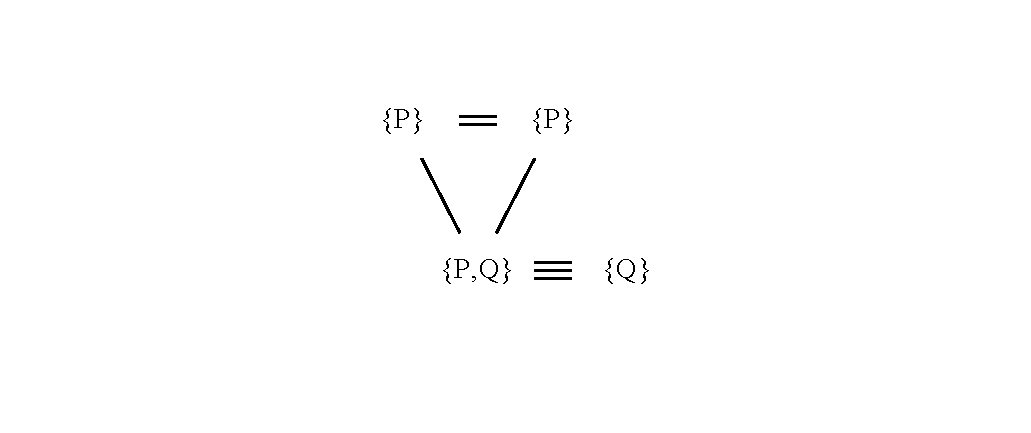
\includegraphics{approximation_example}
\end{figure}

Every model is discernable with respect to the lower approximation, see \ref{def:fully_discernable}.

\begin{definition}[Discernable model]
\label{def:fully_discernable}
\begin{align}
\text{We say that a model is \emph{fully discernable} with respect to a binary relation} \approx \text{iff} \\
\forall x, y \in D (
    [x]_{\approx} = [y]_{\approx}
  \lor
    \mathbb{P}([x]_{\approx}) \neq \mathbb{P}([y]_{\approx})
  )
\end{align}
\end{definition}

So for every binary relation we can give two discernability relations, plus a boundary in between. See figure \ref{fig:indiscernibility_example} for an example.

\begin{figure}
\label{fig:indiscernibility_example}
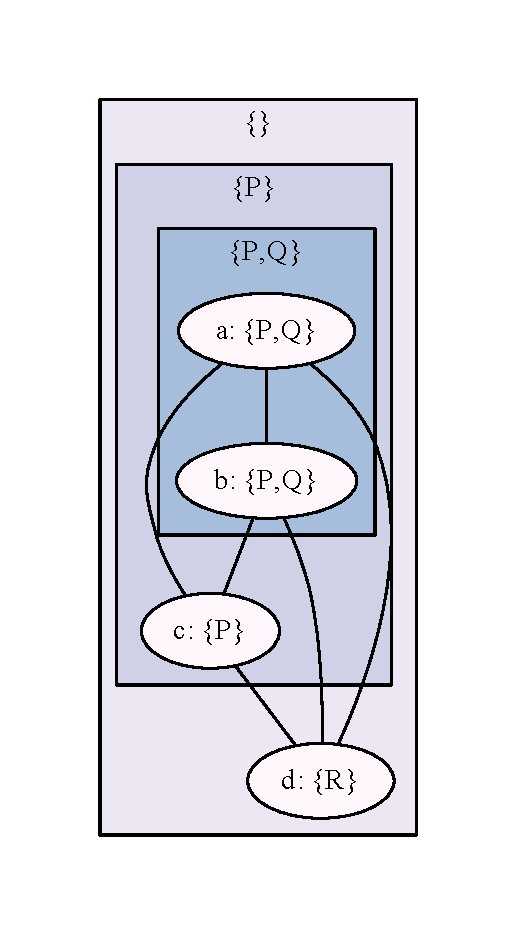
\includegraphics{indiscernibility_example}
\end{figure}





\begin{comment}
\section{Approach II}

How to handle:
\begin{itemize}
\item \textbf{Properties of arbitrary depth.} Properties can have arbitrary
      depth. For instance I am living in a city that is located in a country
      that is part of the European Union. Deep properties traverse
      (non-linked) resources or blank nodes.
\item \textbf{Property hierarchy} Should subproperties be treated
      as separate properties, not at all, or in a special way?
\item \textbf{Graphyness} An RDF graph is assumed to be a `real' graph,
      i.e., RDF properties cannot be RDF nodes.
\end{itemize}

We are given an equivalence relation $\approx$ which is induced from the given set of triples. The properties that are used to construct the quivalence relation can be freely chosen, although obvious choices involve \emph{owl:sameAs}, \emph{skos:somewhatKindaSimila}.

The universe of discourse $\mathbb{U}$ consists of the RDF nodes that appear
in the given triples.

We define a mapping from partition members onto $\mathcal{P}(\mathbb{P})$,
where $\mathbb{P}$ are the properties that occur in the given set of triples.
\footnote{Here we assume that no property is an RDF node.}

\begin{definition}[Predicates]
\begin{eqnarray}
f^{+}_{\mathbb{P}}([x]_{\approx}) = \{ P &\vert&
    \exists y_1 \in [x]_{\approx}, \exists z_1 (y_1Pz_1 \land \\
    & & \  \forall y_2 \in [x]_{\approx} \setminus \{ y_1 \},
    \exists z_2 (y_2Pz_2 \rightarrow z_1 = z_2))) \} \nonumber
\end{eqnarray}
\end{definition}

Partition members are grouped based on a similarity metric.
We choose the Jaccard index for this, but the choise for the combination
of metrics and approximation values is arbitrary.

\begin{definition}[Groups]
\begin{equation}
[y]_{\approx} \in G_{[x]_{\approx}} \  \text{iff} \ 
\frac{\vert f_{\mathbb{P}}([x]_{\approx}) \cap f_{\mathbb{P}}([y]_{\approx}) \vert}
     {\vert f_{\mathbb{P}}([x]_{\approx}) \cup f_{\mathbb{P}}([y]_{\approx}) \vert}
     > c
\end{equation}
\end{definition}

\begin{align}
Jacc(S, T) = \frac{\vert S \cap T) \vert}{\vert S \cup T \vert} \\
Jacc_{\delta}(S, T) = 1 - Jacc(S, T)
\end{align}

\begin{definition}[Groups]
\begin{equation}
G_{[x]_{\approx}} = \{ [y]_{\approx} \  \vert \ 
  Jacc(f^{+}_{\mathbb{P}}([x]_{\approx}), f^{+}_{\mathbb{P}}([y]_{\approx})) > c_1
  \  \land \ 
  Jacc_{\delta}(f^{+}_{\mathbb{P}}([x]_{\approx}), f^{+}_{\mathbb{P}}([y]_{\approx})) < c_2
\end{equation}
\end{definition}

\begin{definition}
\begin{equation}
G_{\approx} = \{ G_{[x]_{\approx}} \  \vert \  x \in \mathbb{U} \}
\end{equation}
\end{definition}

Based on the definition of groups we can identify the indiscernability
properties that characterize a collection of similar partition members.

\begin{definition}[Indiscernability]
\begin{equation}
\text{The members of} \  G_{[x]_{\approx}} \  \text{are} \ 
  \underset{
    \substack{x' \in [x]_{\approx}}
  }{
    \operatorname{\bigcap}
  }
  f^{+}_{\mathbb{P}}([x']_{\approx})
  \text{-indiscernable}.
\end{equation}
\end{definition}

We define the indiscernability set for a partition member as follows:

\begin{definition}[Indiscernability]
\begin{equation}
f_{\mathbb{I}}([x]_{\approx}) =
  \langle
    \bigcap_{y \in G_{[x]_{\approx}}} f^{+}_{\mathbb{P}}(y),
    \bigcap_{y \in G_{[x]_{\approx}}} f^{-}_{\mathbb{P}}(y)
  \rangle
\end{equation}
\end{definition}

What is special about this approach is that we define (in)discernability on
the level of equivalence sets over individuals,
where normally this is defined on the level of individuals.

Observe that we are not talking about sets of indiscernable instances
(as in traditional approaches towards identity),
but about \emph{indiscernability descriptions}
(in terms of domain properties).
This means that $[x]_f([x]_{\approx}) = [x]_{\approx}$ is not true for the
general case. So for each group there can be instances in $[x]_{\approx}$
but not in $G_{[x]_{\approx}}$
(depending on the similarity strictures chosen).
But there can also be instances in $G_{[x]_{\approx}}$ that are not in
$[x]_{\approx}$.

\begin{definition}
\begin{equation}
\approx' = \{ \langle x, y \rangle \in \mathbb{U}^2 \  \vert \ 
    \forall P \in i_1(f_{\mathbb{I}}([x]_{\approx})), \exists z (xPz \leftrightarrow yPz) \}
\end{equation}
\end{definition}
\end{comment}





\section{Rough set theory}
\label{sec:rough_set_theory}

In our case the domain is consists of pairs and the attributes are composed, see \ref{eq:rough_set}. Assume that $\forall a,b \in A (V_a = V_b)$, we can give the composite function for $a^*$.

\begin{align}
\label{eq:rough_set_classic}
U \\
A \\
\forall a^* \in A^* (U \rightarrow V_a) \\
\forall P \subseteq A (
    IND(P) = \{
      \langle x, y \rangle
    \  \vert \ 
      \forall a \in P (a(x) = a(y))
    \}
  )
\end{align}

\begin{align}
\label{eq:rough_set_generic}
U^* = U^n \\
A* = \mathcal{P}(A) \\
\forall a^* \in A^* (U^* \rightarrow V_a) \\
a^*(x_1, \ldots, x_n) \  \text{iff} \  \forall a \in a^* (a(x_1) = \ldots = a(x_n))
\end{align}

We will only consider cases in which $n = 2$ and $V_a = \{ 0, 1 \}$. \ref{eq:rough_set_specific} defines the indiscernability function that we use, where $P^* \subseteq A^*$.

\begin{definition}[Binary indiscernability]
\begin{align}
\label{eq:rough_set_specific}
IND(P^*) = \{
  \langle
    \langle x_1, y_1 \rangle,
    \langle x_2, y_2 \rangle
  \rangle \in (U^2)^2
\  \vert \ 
  \langle x_1, y_1 \rangle P^* \langle x_2, y_2 \rangle
\}
\end{align}
\end{definition}

In the following we shall only consider cases in which $P^* = A^*$. This partitions $U^2$ into sets of pairs that are $P^*$-indiscernible for the same predicate sets that occur in $\mathcal{P}(A^*)$ (see definition \ref{eq:rough_set_specific} for binary indiscernability).

\begin{definition}[Binary indiscernability]
\begin{align}
\label{eq:rough_set_r}
\langle x_1, y_1 \rangle P^* \langle x_2, y_2 \rangle \  \text{iff} \  \\
  \forall a^* \in P^* (
    (x_1 \in \bigcap a^* \leftrightarrow y_1 \in \bigcap a^*)
  \leftrightarrow
    (x_2 \in \bigcap a^* \leftrightarrow y_2 \in \bigcap a^*)
  )
\end{align}
\end{definition}

\section{Evaluation}
\label{sec:evaluation}

Take a $sameAs$ relation and a $related$ relation defined over the same domain. Merge them together into a new relation $\approx$. Establish the lower and higher approximation of $\approx$. The hypothesis is that the boundary overlap with $related$ is bigger as a percentage of the size of $related$ than the boundary overlap with $sameAs$ as a percentage of the size of $sameAs$.

Take a set of alignment pairs with a certain probability between $0.0$ and $1.0$. Choose an arbitrary cutoff point, e.g. $0.7$. Define $\approx$ as those alignment pairs that have probability larger than $0.7$. The first hypothesis is that the alignments with probability between (arbitrary choice) $0.6$ and $0.7$ are in the higher approximation. The second hypothesis is that the alignments that have probability between $0.7$ and (arbitrarily chosen) $0.8$ are in the lower approximation.

Take a set of automatically retrieved alignments pairs with probability attached. Take the gold standard for this alignment exercise (i.e., having probability $1.0$ for each pair). The hypothesis is that the lower approximation of the automated alignments is in the gold standard.

\end{document}

